\chapter{tex笔记}
%%%%%%%%%%%%%%%%%%%%%%%%%%%%%%%%%%%%%%%%%%%%%%%
%%%%%%%%%%%%%%%%%%%%%%%%%%%%%%%%%%%%%%%%%%%%%%%
\section{使用频率较低的符号列表}

\tcbset{skin=enhanced, fonttitle=\bfseries, boxrule=1mm, drop fuzzy shadow}
\begin{tcblisting}{title=特殊符号表}
 \begin{center}
  \begin{tabular}{|c|c|c|c|c|}
    \hline
    $\hbar$ & $\imath$ & $\jmath$ & $\ell$ & $\Im$\\
    \hline
    $\wp$ & $\mho$ & $\prime$ & $\Box$ & $\Diamond$\\
    \hline
    $\bot$ & $\top$ & $\surd$ & $\diamondsuit$ & $\heartsuit$\\
    \hline
    $\clubsuit$ & $\spadesuit$ & $\neg$ & $\lnot$ & $\flat$\\
    \hline
    $\natural$ & $\sharp$ & \dag & \ddag & \S\\
    \hline
    \P & \copyright & \pounds & \textregistered & \\
    \hline
  \end{tabular}
\end{center}
\end{tcblisting}
%%%%%%%%%%%%%%%%%%%%%%%%%%%%%%%%%%%%%%%%%%%%%%%
%%%%%%%%%%%%%%%%%%%%%%%%%%%%%%%%%%%%%%%%%%%%%%%
\section{itemize enumerate}
\begin{tcblisting}{title=列表}
  \begin{enumerate}
  \item This is an example of \ldots
  \item \ldots the usual enumeration.
  \begin{enumerate}[a)]
    \item And this is a \ldots
    \item \ldots couple of \ldots
  \end{enumerate}
    \item 
    \begin{enumerate}[-- i --]
    \item \ldots examples of \ldots
    \item \ldots custom-tailored \ldots
    \item \ldots enumerations.
    \newcounter{enumii_saved}
    \setcounter{enumii_saved}{\value{enumii}}
    \end{enumerate}
    Some general comments
    \begin{enumerate}[-- i --]
    \setcounter{enumii}{\value{enumii_saved}}
    % 如果要换另一个条列式项目, 但编号接续, 使用\newcounter{enumii_saved}来操作
    \item My next point.
    \setcounter{enumii}{7}
    % 使用setcounter{enumii}{数字}来指定编号号码
    \item My eighth point.
    \end{enumerate}
  \end{enumerate}
\end{tcblisting}
%%%%%%%%%%%%%%%%%%%%%%%%%%%%%%%%%%%%%%%%%%%%%%%
%%%%%%%%%%%%%%%%%%%%%%%%%%%%%%%%%%%%%%%%%%%%%%%
\section{tikz}
\begin{tcblisting}{title=画图}
  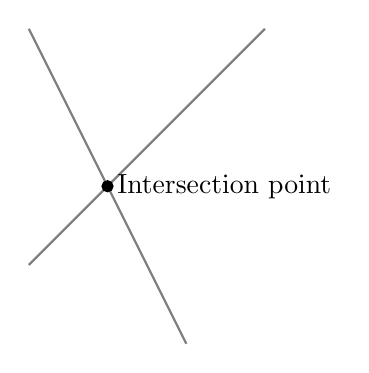
\begin{tikzpicture}
   \draw[gray, thick] (-1,2) -- (1,-2);
   \draw[gray, thick] (-1,-1) -- (2,2);
   \filldraw[black] (0,0) circle (2pt) node[anchor=west] {Intersection point};
  \end{tikzpicture}
  \begin{tikzpicture}
    \draw (-2,0) -- (2,0);
    \filldraw [gray] (0,0) circle (2pt);
    \draw (-2,-2) .. controls (0,0) .. (2,-2);
    \draw (-2,2) .. controls (-1,0) and (1,0) .. (2,2);
  \end{tikzpicture}
  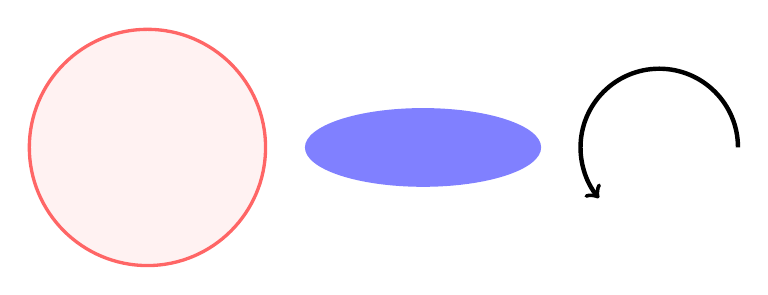
\begin{tikzpicture}
    \filldraw[color=red!60, fill=red!5, very thick](-1,0) circle (1.5);
    \fill[blue!50] (2.5,0) ellipse (1.5 and 0.5);
    \draw[ultra thick, ->] (6.5,0) arc (0:220:1);
  \end{tikzpicture}
\end{tcblisting}

\begin{tcblisting}{title=画图}
  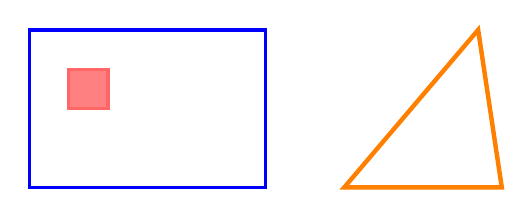
\begin{tikzpicture}
    \filldraw[color=red!60, fill=red!50, very thick](1,1) rectangle (0.5,1.5);
    \draw[blue, very thick] (0,0)rectangle (3,2);
    \draw[orange, ultra thick] (4,0) -- (6,0) -- (5.7,2) -- cycle;
  \end{tikzpicture}
\end{tcblisting}

\begin{tcblisting}{title=270226}
  \definecolor{myred}{RGB}{183,18,52}
  \definecolor{myyellow}{RGB}{254,213,1}
  \definecolor{myblue}{RGB}{0,80,198}
  \definecolor{mygreen}{RGB}{0,155,72}
  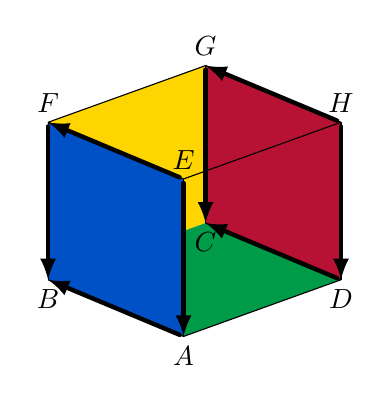
\begin{tikzpicture}[
    line join=round,
    y={(-0.86cm,0.36cm)},x={(1cm,0.36cm)}, z={(0cm,1cm)},
    arr/.style={-latex,ultra thick,line cap=round,shorten <= 1.5pt}
  ]
  \def\Side{2}
  \coordinate (A1) at (0,0,0);
  \coordinate (A2) at (0,\Side,0);
  \coordinate (A3) at (\Side,\Side,0);
  \coordinate (A4) at (\Side,0,0);
  \coordinate (B1) at (0,0,\Side);
  \coordinate (B2) at (0,\Side,\Side);
  \coordinate (B3) at (\Side,\Side,\Side);
  \coordinate (B4) at (\Side,0,\Side);

  \fill[myyellow] (A2) -- (A3) -- (B3) -- (B2) -- cycle;
  \fill[mygreen]  (A2) -- (A3) -- (A4) -- (A1) -- cycle;
  \fill[myred](A3) -- (B3) -- (B4) -- (A4) -- cycle;
  \fill[myblue]   (A1) -- (A2) -- (B2) -- (B1) -- cycle;

  \draw (A2) -- (A1) -- (A4);
  \draw (B2) -- (B1) -- (B4) -- (B3) -- cycle;
  \draw (A1) -- (B1);
  \draw (A2) -- (B2);
  \draw (A4) -- (B4);

  \draw[thin] (A3) -- (B3);
  \draw[thin] (A3) -- (A4);

  \path[arr] 
    (A1) edge (A2)
    (B2) edge (A2)
    (B1) edge (B2)
    (B1) edge (A1)
    (B4) edge (A4)
    (B3) edge (A3)
    (B4) edge (B3)
    (A4) edge (A3);

  \node[below] at (A1) {$A$};
  \node[below] at (A2) {$B$};
  \node[below] at (A3) {$C$};
  \node[below] at (A4) {$D$};
  \node[above] at (B1) {$E$};
  \node[above] at (B2) {$F$};
  \node[above] at (B3) {$G$};
  \node[above] at (B4) {$H$};
  \end{tikzpicture}
\end{tcblisting}

\begin{tcblisting}{title=根据三点画弧}
  \begin{tikzpicture}
    \tkzDefPoint(1,2){A}
    \tkzDefPoint(3,4){B}
    \tkzDefPoint(2,4){C}
    \tkzCircumCenter(A,B,C)\tkzGetPoint{O}
    \tkzDrawArc(O,C)(A)
  \end{tikzpicture}
\end{tcblisting}


\begin{tcblisting}{title=字体}
  $\mathscr{ABCDEFGHIJKLMNOPQRSTUVWXYZ}$\\
  $\mathbb{ABCDEFGHIJKLMNOPQRSTUVWXYZ}$\\
  $\mathcal{ABCDEFGHIJKLMNOPQRSTUVWXYZ}$\\
  $\mathfrak{ABCDEFGHIJKLMNOPQRSTUVWXYZ}$
\end{tcblisting}
